\documentclass{article}
\usepackage[margin=0.5in]{geometry}
\usepackage{graphicx}
\usepackage{multirow}
\usepackage{subcaption}
\usepackage{xcolor} 
\usepackage{sectsty}
\usepackage{listings}
\usepackage{enumitem}
\usepackage{needspace}
\usepackage{amssymb}
\usepackage{adjustbox}
\usepackage{tocloft}
\usepackage{hyperref}

\hypersetup{
    colorlinks=true,
    linkcolor=blue, % Internal links
    urlcolor=blue, % External links
    citecolor=blue, % Citations
}

\renewcommand{\cftsecleader}{\cftdotfill{\cftdotsep}} % Adds dots between sections and page numbers
\setlength{\cftbeforesecskip}{0.5em} % Adjusts space before sections in the table of contents
\setlength{\cftsecindent}{0em} % Adjusts indentation for sections in the table of contents
\setlength{\cftsecnumwidth}{2.5em} % Adjusts width for section numbers in the table of contents

% Customization of itemize environments
\setlist[itemize]{label=$\bullet$, topsep=0.5em, itemsep=0em, leftmargin=*} % Adjusts itemize environment formatting

% Define a light gray color for code background
\definecolor{light-gray}{gray}{0.95}

% Define a new environment for code display
\lstnewenvironment{cppcode}[1][]{
    \lstset{
        backgroundcolor=\color{light-gray},
        frame=lines,
        basicstyle=\ttfamily,
        breaklines=true,
        columns=fullflexible,
        postbreak=\mbox{\textcolor{red}{$\hookrightarrow$}\space},
        captionpos=b,
        #1 % Additional options for listings can be passed here
    }
}{}

\definecolor{codebackground}{rgb}{0.95,0.95,0.95}
\definecolor{commentgreen}{RGB}{34,139,24}

\lstset{
    language=C++,
    backgroundcolor=\color{codebackground},
    basicstyle=\large\ttfamily,
    commentstyle=\color{commentgreen},
    keywordstyle=\color{blue},
    stringstyle=\color{purple}, % Color for strings
    numbers=left,
    numberstyle=\tiny\color{brown},
    stepnumber=1,
    numbersep=5pt,
    frame=tb,
    captionpos=b,
    breaklines=true,
    breakatwhitespace=true,
    tabsize=4,
    % Custom colors for brackets using literate
    literate=
        {<}{{\textcolor{green}{<}}}1
        {-}{{\textcolor{green}{-}}}1
        {>}{{\textcolor{green}{>}}}1
        {[}{{\textcolor{orange}{[}}}1
        {]}{{\textcolor{orange}{]}}}1
        {\{}{{\textcolor{blue}{\{}}}1
        {\}}{{\textcolor{blue}{\}}}}1
}


\title{\Huge Assignment 8-Multilevel Queue Scheduling}
\author{22000021}
\date{\today}
 
\begin{document}
\maketitle
\newpage

\tableofcontents
\newpage

\section{Introduction}

Your introduction is quite comprehensive and covers all the essential aspects of the code. However, if you'd like to enhance it further, you might consider incorporating a bit more detail or emphasizing specific points. Here's a slightly refined version of your introduction:

This program serves as a simulation of a multilevel queue scheduling algorithm, a critical component in the realm of operating system design. It organizes processes into priority-based queues, with four distinct queues labeled q0 to q3. Each queue is assigned a unique scheduling strategy tailored to its priority level: 
\begin{center}
  \begin{description}
      \item Round Robin (RR): Scheduling for q0
      \item Shortest Job First (SJF): Scheduling for q1 and q2
      \item First-In-First-Out (FIFO): Scheduling for q3
  \end{description}
\end{center}  
The time quantum for each queue is set at 20 seconds, after which the CPU switches between queues to execute processes. By prompting users to input the number of processes and their priorities for each queue, the program facilitates dynamic simulation scenarios. The primary objective of this simulation is to analyze the efficiency and performance of various scheduling algorithms under varying workload conditions. This analysis aims to provide valuable insights into optimizing system scheduling strategies for enhanced operational efficiency.


\section{Methodology}
\vspace{\baselineskip}
The Methodology section of this report delves into the implementation details of the provided C code, which revolves around process and queue management. The code is designed to simulate a multilevel queue scheduling algorithm, a fundamental aspect of operating system design. The methodology is organized into several subsections, each focusing on different aspects of the code's implementation. These subsections include Process Implementation, which covers the structure and properties of processes; Queue Operations, detailing the functions for queue management such as enqueue, dequeue, and queue status checks; and Process Initialization, explaining how processes are initialized and added to the corresponding queues based on user input. Through a comprehensive exploration of these components, this report aims to provide a thorough understanding of the code's functionality and its relevance in the context of process and queue management in operating systems.

\subsection{Process Implementation}
\vspace{\baselineskip}
The multilevel queue scheduling algorithm is implemented using \textbf{C++}’s class-based approach.
The ’Process’ structure represents a process with properties such as process ID, burst time, remaining time, wait time Turnaround time. 
The ’Queue’ structure represents a queue with properties such as front, rear, and an array to hold the processes
For the implementation purpose, I have used the maximum number of processes in the queue as 100
\\
\begin{lstlisting}
#define MAX_SIZE 100

struct Process{
    int Id;                                
    int BurstTime;                        
    int RemainingTime;                    
    int WaiteTime;                        
    int TurnaroundTime;                   
};

struct Queue{                             
    int Rear;                             
    int Front;                            
    struct Process* list[MAX_SIZE];       
};

int time=0;

\end{lstlisting}

\begin{enumerate}[label=\textbf{\arabic*.}]
  \item \texttt{MAX\_SIZE}: Defines the maximum number of processes that the program can handle.
  
  \item \texttt{struct Process}:
  \begin{itemize}[label=--]
      \item \texttt{Id}: Represents the unique identifier or ID of the process.
      \item \texttt{BurstTime}: Indicates the time taken by the process to execute or its burst time.
      \item \texttt{RemainingTime}: Represents the remaining time needed for the process to complete its execution.
      \item \texttt{WaitTime}: Stores the total waiting time of the process.
      \item \texttt{TurnaroundTime}: Stores the total time taken for the process from submission to completion.
  \end{itemize}
  
  \item \texttt{struct Queue}:
  \begin{itemize}[label=--]
      \item \texttt{Rear}: Represents the rear index of the queue.
      \item \texttt{Front}: Represents the front index of the queue.
      \item \texttt{list[MAX\_SIZE]}: An array of pointers to \texttt{Process} structures.
  \end{itemize}
  
  \item \texttt{int time}: Keeps track of the global time in the program.
\end{enumerate}

\vspace{1\baselineskip}
\subsection{Queue Operations}
\vspace{\baselineskip}

The code segment encapsulates essential functionalities for managing processes within a queue and scheduling algorithms.\\
The IsEmpty and IsFull functions ascertain the status of the queue, determining whether it is empty or full, crucial for maintaining queue integrity during enqueue and dequeue operations.\\
Enqueue and Dequeue functions handle the insertion and deletion of processes from the queue, respectively, ensuring proper queue management. Additionally.\\
The MIN function identifies the process with the minimum remaining time in the queue, facilitating scheduling decisions.\\
Index\textunderscore{}Dequeue function further refines dequeue operations by allowing removal of processes at specific index in the queue.\\
These functions collectively form the backbone of process and queue management, essential for implementing efficient scheduling strategies and ensuring smooth program execution.\\


\begin{lstlisting}
bool IsEmpty(struct Queue* Q) {                                 
  return ((Q->Front==-1)||(Q->Rear==-1));
}


bool IsFull(struct Queue* Q) {                                  
  return (Q->Rear+1)%MAX_SIZE==Q->Front;
}


void Enqueue(struct Queue* Q,struct Process* p){                 
    if(IsFull(Q)){
        printf("No space in the Queue\n");
    }
    else{
        if(IsEmpty(Q)){
            Q->Front=0;
        }
        Q->Rear=(Q->Rear+1)%MAX_SIZE;
        Q->list[Q->Rear]=p;
    }
}
\end{lstlisting}
\newpage
\begin{lstlisting}[caption={Queue Operations}, label={lst:queue_operations},firstnumber=23]
void Dequeue(struct Queue* Q){                                   
    if(IsEmpty(Q)){
        printf("The Queue is empty\n");
    }
    else{
        if(Q->Rear==Q->Front){
            Q->Rear=-1;
            Q->Front=-1;
        }
        else{
            Q->Front=(Q->Front+1)%MAX_SIZE;
        }
    }
}


int MIN(struct Queue* Q){
    if(IsEmpty(Q)){
        return -1;
    }
    int min_Index=Q->Front;
    for(int i=Q->Front;i<=Q->Rear;i++){
        if(Q->list[min_Index]->RemainingTime>Q->list[i]->RemainingTime){
            min_Index=i;
        }
    }
    return min_Index;
}


void Index_Dequeue(struct Queue *Q,int index){
    if(IsEmpty(Q)){
        return;
    }
    else{
        if(index==Q->Front){
            Dequeue(Q);
        }
        else{
            for(int i=index;i>Q->Front;i--){
                Q->list[i]=Q->list[i-1];
            }
            Q->Front++;
        }
    }
}
\end{lstlisting}

\newpage
Enqueue and Dequeue are the same operations following a circular queue.delete is a variation of dequeue, where the dequeued process will be enqueued to the same queue.

\vspace{\baselineskip}
\subsection{Process initialization}
\vspace{\baselineskip}

For the code to work without any interrupts we ask for the user to enter the count of the process that will be processed In c++ we cant do that without user inputs 
The code for initialization of the process after the detail for the process has been input we store the process temporarily to a user define variable and than that process is added to the corresponding queue

\begin{lstlisting}
int n;
    printf("Enter the number of process to enter =");
    scanf("%d",&n);
    printf("\n");

    struct Queue Q0 = {.Rear = -1, .Front = -1};
    struct Queue Q1 = {.Rear = -1, .Front = -1};
    struct Queue Q2 = {.Rear = -1, .Front = -1};
    struct Queue Q3 = {.Rear = -1, .Front = -1};

    for(int i=0;i<n;i++){
        int k;
        struct Process* P=(struct Process*) malloc (sizeof(struct Process));
        printf("Enter the process Id =");
        scanf("%d",&P->Id);
        printf("Enter the burst time of the process =");
        scanf("%d",&P->BurstTime);
        P->RemainingTime=P->BurstTime;
        printf("Enter the priority of the process=");
        scanf("%d",&k);
        printf("\n");
        while(k<0 || k>4){                                                               //To check the priority of the process
            printf("Priority is wrong. Enter again: ");
            scanf("%d",&k);
            printf("\n");
        }
        if(k==0){
            Enqueue(&Q0,P);
        }
        else if(k==1){
            Enqueue(&Q1,P);
        }
        else if(k==2){
            Enqueue(&Q2,P);
        }
        else if(k==3){
            Enqueue(&Q3,P);
        }
    }
\end{lstlisting}

\newpage
This part of the code initializes four separate queues (Q0, Q1, Q2, and Q3) representing different priority levels in a multilevel queue scheduling algorithm. It first prompts the user to input the number of processes to enter. Then, it iterates n times to input details for each process, such as process ID, burst time, and priority.
During each iteration, memory is dynamically allocated for a new Process. The user is prompted to enter the process details, and the entered information is assigned to the respective members of the Process.
The priority of the process is checked to ensure it falls within the valid range of 0 to 3. If the priority is valid, the process is enqueued into the corresponding queue (Q0, Q1, Q2, or Q3) using the Enqueue() function.
Overall, this section of the code facilitates the dynamic creation and enqueuing of processes into their respective priority-based queues based on user input.

\vspace{\baselineskip}
\section{Scheduling Algorithm}
\vspace{\baselineskip}
\subsection{RR (Round Robin) Scheduling Algorithm}
\begin{itemize}
    \item The function determines the quantum slice by dividing the total number of processes in the queue by the time quantum of the multilevel queue. This ensures fair distribution of time among processes.
    \item if the processes in the queue is greater than 20 seconds we cant use decimal time to execute a process there is a exception when that happens
    \item It enters a loop that iterates until the quantum slice is exhausted. This loop handles cases where the quantum slice is smaller than the Robin slice or vice versa.
    \item If a process's remaining time is less than or equal to the Robin slice, the process completes its execution. It is removed from the queue, and the global time is updated. A message indicating the process ID and exit time is printed
    \item If a process's remaining time exceeds the Robin slice, the Robin slice is subtracted from its remaining time, and the global time is updated accordingly. The process remains in the queue for further execution
    \item This process continues until the quantum slice is exhausted or the queue becomes empty.
\end{itemize}

\begin{lstlisting}[basicstyle=\footnotesize]

void RR(struct Queue* Q){ 
  int timeQuantum=20/size;
  printf("timeQuantum =%d\n",timeQuantum);
  for(int i=Q->Front;i<=Q->Rear;i++){
    if(Q->list[i]->RemainingTime<=timeQuantum){
      int t=time;
      time=time+Q->list[i]->RemainingTime;
      printf("Process %d executed from time %d to %d\n", Q->list[i]->Id,t,time);
      Q->list[i]->TurnaroundTime=time;
      Q->list[i]->WaiteTime=Q->list[i]->TurnaroundTime-Q->list[i]->BurstTime;
      printf("The waiting time of the process =%d\n",Q->list[i]->WaiteTime);
      printf("The turnaround time of the process =%d\n\n",Q->list[i]->TurnaroundTime);
      Index_Dequeue(Q,i);
    } 
    else{
      int t=time;
      time=time+timeQuantum;
      printf("Process %d executed from time %d to %d\n", Q->list[i]->Id,t,time);
      Q->list[i]->RemainingTime=Q->list[i]->RemainingTime-timeQuantum;
      printf("There is a remaining burst time of %d\n\n",Q->list[i]->RemainingTime);
    }   
  }
}
\end{lstlisting}

\vspace{\baselineskip}
\subsection{SJF (Shortest Job First) Scheduling Algorithm}
\begin{itemize}
    \item According to the arrival time and the shortest job in the queue at the moment gets executed without being preemption.
    \item Selecting the Shortest Job: The scheduler selects the process with the shortest burst time from the pool of available processes.
    \item It prioritizes processes based on their burst time, where the process with the shortest burst time is given preference for execution.
    \item Executing the Process: Once selected, the chosen process is dispatched for execution on the CPU. The CPU executes the process until it completes its entire burst time.
\end{itemize}
\vspace{\baselineskip}
\subsection{FIFO (First In First Out) Scheduling Algorithm}
\begin{itemize}
    \item The process are executed in the order they are enqueued into the Queue just how the Queue algorithm works
\end{itemize}

\newpage
\section{Pros and Cons of Scheduling Algorithms}
\begin{table}[h]
  \centering
  \resizebox{\textwidth}{!}{
      \setlength{\arrayrulewidth}{2pt}
      \setlength{\tabcolsep}{15pt}
      \begin{tabular}{|p{3cm}|p{6cm}|p{6cm}|}
      \hline
      \textbf{Algorithm} & \textbf{Pros} & \textbf{Cons} \\
      \hline
      \multirow{3}{*}{RR} 
      & \begin{itemize}
          \item No starvation.
          \item Time-sharing systems.
          \item Every process gets a chance to execute.
        \end{itemize}
      & \begin{itemize}
          \item High context switches.
          \item Poor performance for long running processes.
          \item Becomes FIFO if the time quantum is very high.
        \end{itemize} \\
      \hline
      \multirow{3}{*}{SJF} 
      & \begin{itemize}
          \item Minimizes average waiting time.
          \item Provides better system throughput.
        \end{itemize}
      & \begin{itemize}
          \item Requires knowledge of burst times in advance.
          \item May suffer from high overhead in the presence of frequent arrivals of short jobs.
        \end{itemize} \\
      \hline
      \multirow{3}{*}{FIFO} 
      & \begin{itemize}
          \item Simple and easy to implement.
          \item Suitable for batch processing systems.
          \item Ensures fairness in First Come First serve idea.
        \end{itemize}
      & \begin{itemize}
          \item May suffer from convoy effect.
          \item Poor performance in interactive systems with varying job sizes.
          \item potentially higher average waiting times.
        \end{itemize} \\
      \hline
      \end{tabular}
  }
\end{table}


\section{Results}
This example covers the execution of the 4 queues. The time quantum in the example is taken as 8 for the sake of simplicity
\begin{table}[htbp]
  \centering
  \begin{tabular}{|c|c|c|c|}
      \hline
      \textbf{Process ID} & \textbf{Priority Number} & \textbf{Burst Time (s)} \\
      \hline
      P1 & 0 & 9 \\
      P2 & 0 & 3 \\
      P3 & 1 & 4 \\
      P4 & 1 & 3 \\
      P5 & 1 & 2 \\
      P6 & 2 & 1 \\
      P7 & 2 & 13 \\
      P8 & 2 & 6 \\
      P9 & 3 & 2 \\
      P10 & 3 & 4 \\
      P11 & 3 & 5 \\
      \hline
  \end{tabular}
  \caption{Process Information}
  \label{tab:process_info}
\end{table}

\begin{figure}[t!]
  \centering
  \begin{subfigure}[b]{0.45\textwidth}
    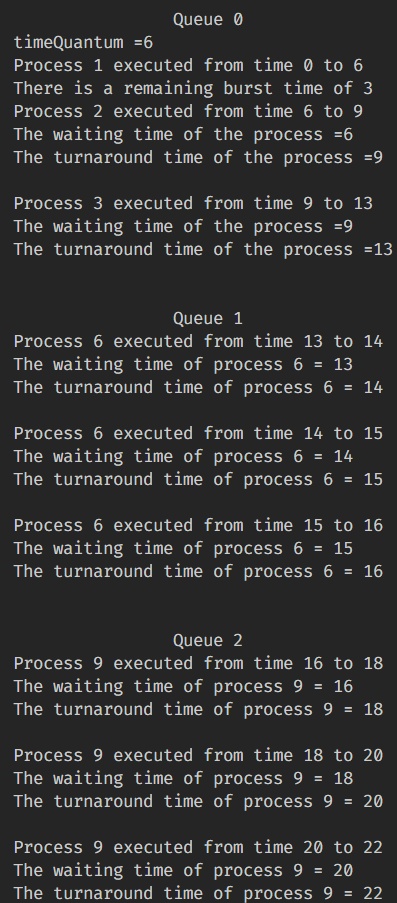
\includegraphics[width=\textwidth]{5.png}
    \caption{Queue 1}
    \label{fig:queue1}
  \end{subfigure}
  \hfill
  \begin{subfigure}[b]{0.45\textwidth}
    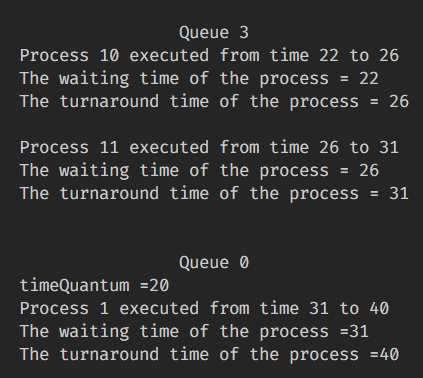
\includegraphics[width=\textwidth]{6.png}
    \caption{Queue 2}
    \label{fig:queue2}
  \end{subfigure}
  \caption{Code output}
  \label{fig:both_queues}
\end{figure}

\clearpage
\newpage
\section{Conclusion}
\subsection{Round Robin Scheduling Algorithm}
\begin{itemize}
  \item Setting the quantum too short produces the worst results, it increases the overhead.
  \item Higher average turnaround time than than SJF but better response.
  \item Turnaround time heavily depends on time quantum. It decreases if majority of burst time is lesser than the time quantum.
  \item Can be used for batch processing in multilevel queue.
  \item No starvation
\end{itemize}

\subsection{Shortest Job First Scheduling Algorithm}
\begin{itemize}
  \item Produces the optimal average turnaround time among these scheduling algorithms.
  \item If shorter jobs keep getting enqueued then aging has to be implemented to prevent starvation.
  \item Turnaround time heavily depends on time quantum. It decreases if majority of burst time is lesser than thetime quantum.
  \item Cannot be implemented at the level of short-term CPU scheduling.
  \item Can be used for interactive processing in multilevel queue.
\end{itemize}

\subsection{First In First Out Scheduling Algorithm}
\begin{itemize}
  \item Has low scheduling overhead because it does not require frequent context switches or involve complex scheduling decisions.
  \item Processes with shorter burst time will have to wait for an unreasonable time if processes with largest burst time arrive before it.
  \item Favours CPU bound processes than I/O bound processes.
  \item Perfect for processes with workloads with no strict time constraint.
  \item Can be used for system processing in multilevel queue.
\end{itemize}

\subsection{Multi Level Queue Scheduling Algorithm}
\begin{itemize}
  \item Overhead is low because the scheduler needs to only select the appropriate queue.
  \item Fairness is present in this algorithm.
  \item Processes in the lower levels face the starvation problem.
\end{itemize}

\section{Program Limitations}
The current version of the program assumes that all process arrivals occur at time 0. However, the program does not account for instances where processes can arrive at different times. This limitation prevents us from obtaining accurate results, such as waiting time and turnaround time, when different processes are enqueued at different times.

The quantum decision during the selection of the Round Robin time quantum has a significant impact. Choosing a static time quantum can lead to worse performance. Instead, we implemented a dynamic approach by using the time quantum from the multilevel queues. Although not perfect, this dynamic implementation produces better results compared to the static implementation.
When the Queue for round robin has more than 20 process only the first 20 process get 1 second to execute other process doesn't gets executed
\end{document}
